\documentclass[10pt]{beamer}
\usetheme{Rochester}

% load syscop style
\usepackage{style/syscop}

%--------------------------------------------------
% TITLE
%--------------------------------------------------

% NOTE: what's in [ ] goes to footer for the fields title, author and date
\title[Real Time Operating Systems Lab]{ Real Time Operating Systems Lab}
\author {Akash John Subash, Tobias Seufert, Prof. Dr Christoph Scholl}
\institute {Chair of Operating Systems}
%--------------------------------------------------
% Usefull packages
%--------------------------------------------------

\usepackage{mathtools}
\usepackage{graphicx}

%\usepackage{style/dimitris}

\begin{document}

% EDF API
\begin{frame}{\small{EDF APIs}}
	\footnotesize{
		 The user Application Program interface (API) to use the Earliest Deadline First (EDF) scheduler implmented in user space consists of invoking the C functions in the folllowing order:\\
	\begin{itemize}
		\item[$\bullet$] $EdfScheduleInit(PeriodicTaskArray, AperiodicTaskArray)$\\
		\item[$\bullet$] $EdfScheduleStart()$\\
		\item[$\bullet$] $EdfDeleteAllTasks()$\\
	\end{itemize}

	 PeriodicTaskArray and AperiodicTaskArray are arrays of the public Task Control Block (TCB) structure $pubTCB\_t$, which along with the above function prototypes are defined in $edf\_scheduler.h$\\
	}%end footnote size	
\end{frame}

\begin{frame}
	\footnotesize{
	Each of the struct elements corresopnding to the following parameters must initilized by the user in PeriodicTaskArray :\\
	\begin{itemize}
		\item[$\bullet$] Period ($P_{i}$) \\
		\item[$\bullet$] Worst case execution time ($c_{i}$) \\
		\item[$\bullet$] Phase ($\phi_{i}$)\\
		\item[$\bullet$] Relative deadline ($D_{i}$)
		\item[$\bullet$] Task number (${i}$)\\
		\item[$\bullet$] Task function ($\tau_{i}$)\\
	\end{itemize}\\
		
	\hfill\break
	and in AperiodicTaskArray :\\
	\begin{itemize}
		\item[$\bullet$] Relative arrival time ($a_{i}$) \\
		\item[$\bullet$] Worst case execution time  ($c_{i}$)\\
		\item[$\bullet$] Task number (${i}$)\\
		\item[$\bullet$] Task function ($J_{i}$)\\
		\item[$\bullet$] Aperiodicity flag\\
	\end{itemize}
	} %end footnote size	
\end{frame}

% EDF API
\begin{frame}
	\footnotesize{
		 EDF Option 1 using trace APIs and the inbuilt priority based scheduler of $FreeRTOS$ is implemented here based on [1].
		 Periodic tasks priorities are updated just prior to task switching via the $traceTASK\_SWITCHED\_OUT()$ macro [2]. 
		 Here, the TCBs stored in the doubly linked lists are sorted implictly by using the APIs from $list.h$
		 
		 \hfill\break
		 Aperiodic tasks are also scheduled by EDF by using a Total Bandwidth Server (TBS) [3], 
		 which assigns fictitios deadlines to them based on the server Utilitzation factor $U_{s}$, and arrival times $a_{i}$. 
		 The aperiodic tasks are deleted after execution of it's first instace. 

		 \hfill\break
		 Task deadline overflows are monitored every defined tick via the $traceTASK\_INCREMENT\_TICK()$ macro and marked for deletion 
		 in the privately maintained TCB $exTCB\_t$. 
		 These are later deleted during the following priority update stage mentioned above.
		 }%end footnote size	
\end{frame}


% Example 5: 4 periodic, 95% Util
\begin{frame}{\small{EDF results: 4 periodic tasks, 95\% utilization factor}}
	\footnotesize{
	\begin{table}[ht]\label{table5}
		\hskip-6.0cm\begin{tabular}{lcccccl}\toprule
		\hline
		 & ${\tau_{5}}$ & ${\tau_{6}}$ & ${\tau_{7}}$ & ${\tau_{8}}$\\\midrule
		\hline
		${\phi_{i}}$ & 0 & 0 & 0 & 0\\
		$a_{i}$ & 0 & 0 & 0 & 0\\
		$c_{i}$ & 100 & 100 & 100 & 100\\
		$P_{i}$ & 500 & 400 & 400 & 400\\
		$D_{i}$ & 500 & 400 & 400 & 400\\\bottomrule
		\hline
	\end{tabular}
	}%end footnote size	
\end{table}

Utilization factor \\
\hfill\break
$U_{p} = \sum \dfrac{C_{i}}{P_{i}}\\
\hspace{0.2in} = \dfrac{100}{500} + \dfrac{100}{400} + \dfrac{100}{400} + \dfrac{100}{400} = 0.95$
\end{frame}

\begin{frame}
	\footnotesize{
	\begin{figure*}
		\centerline{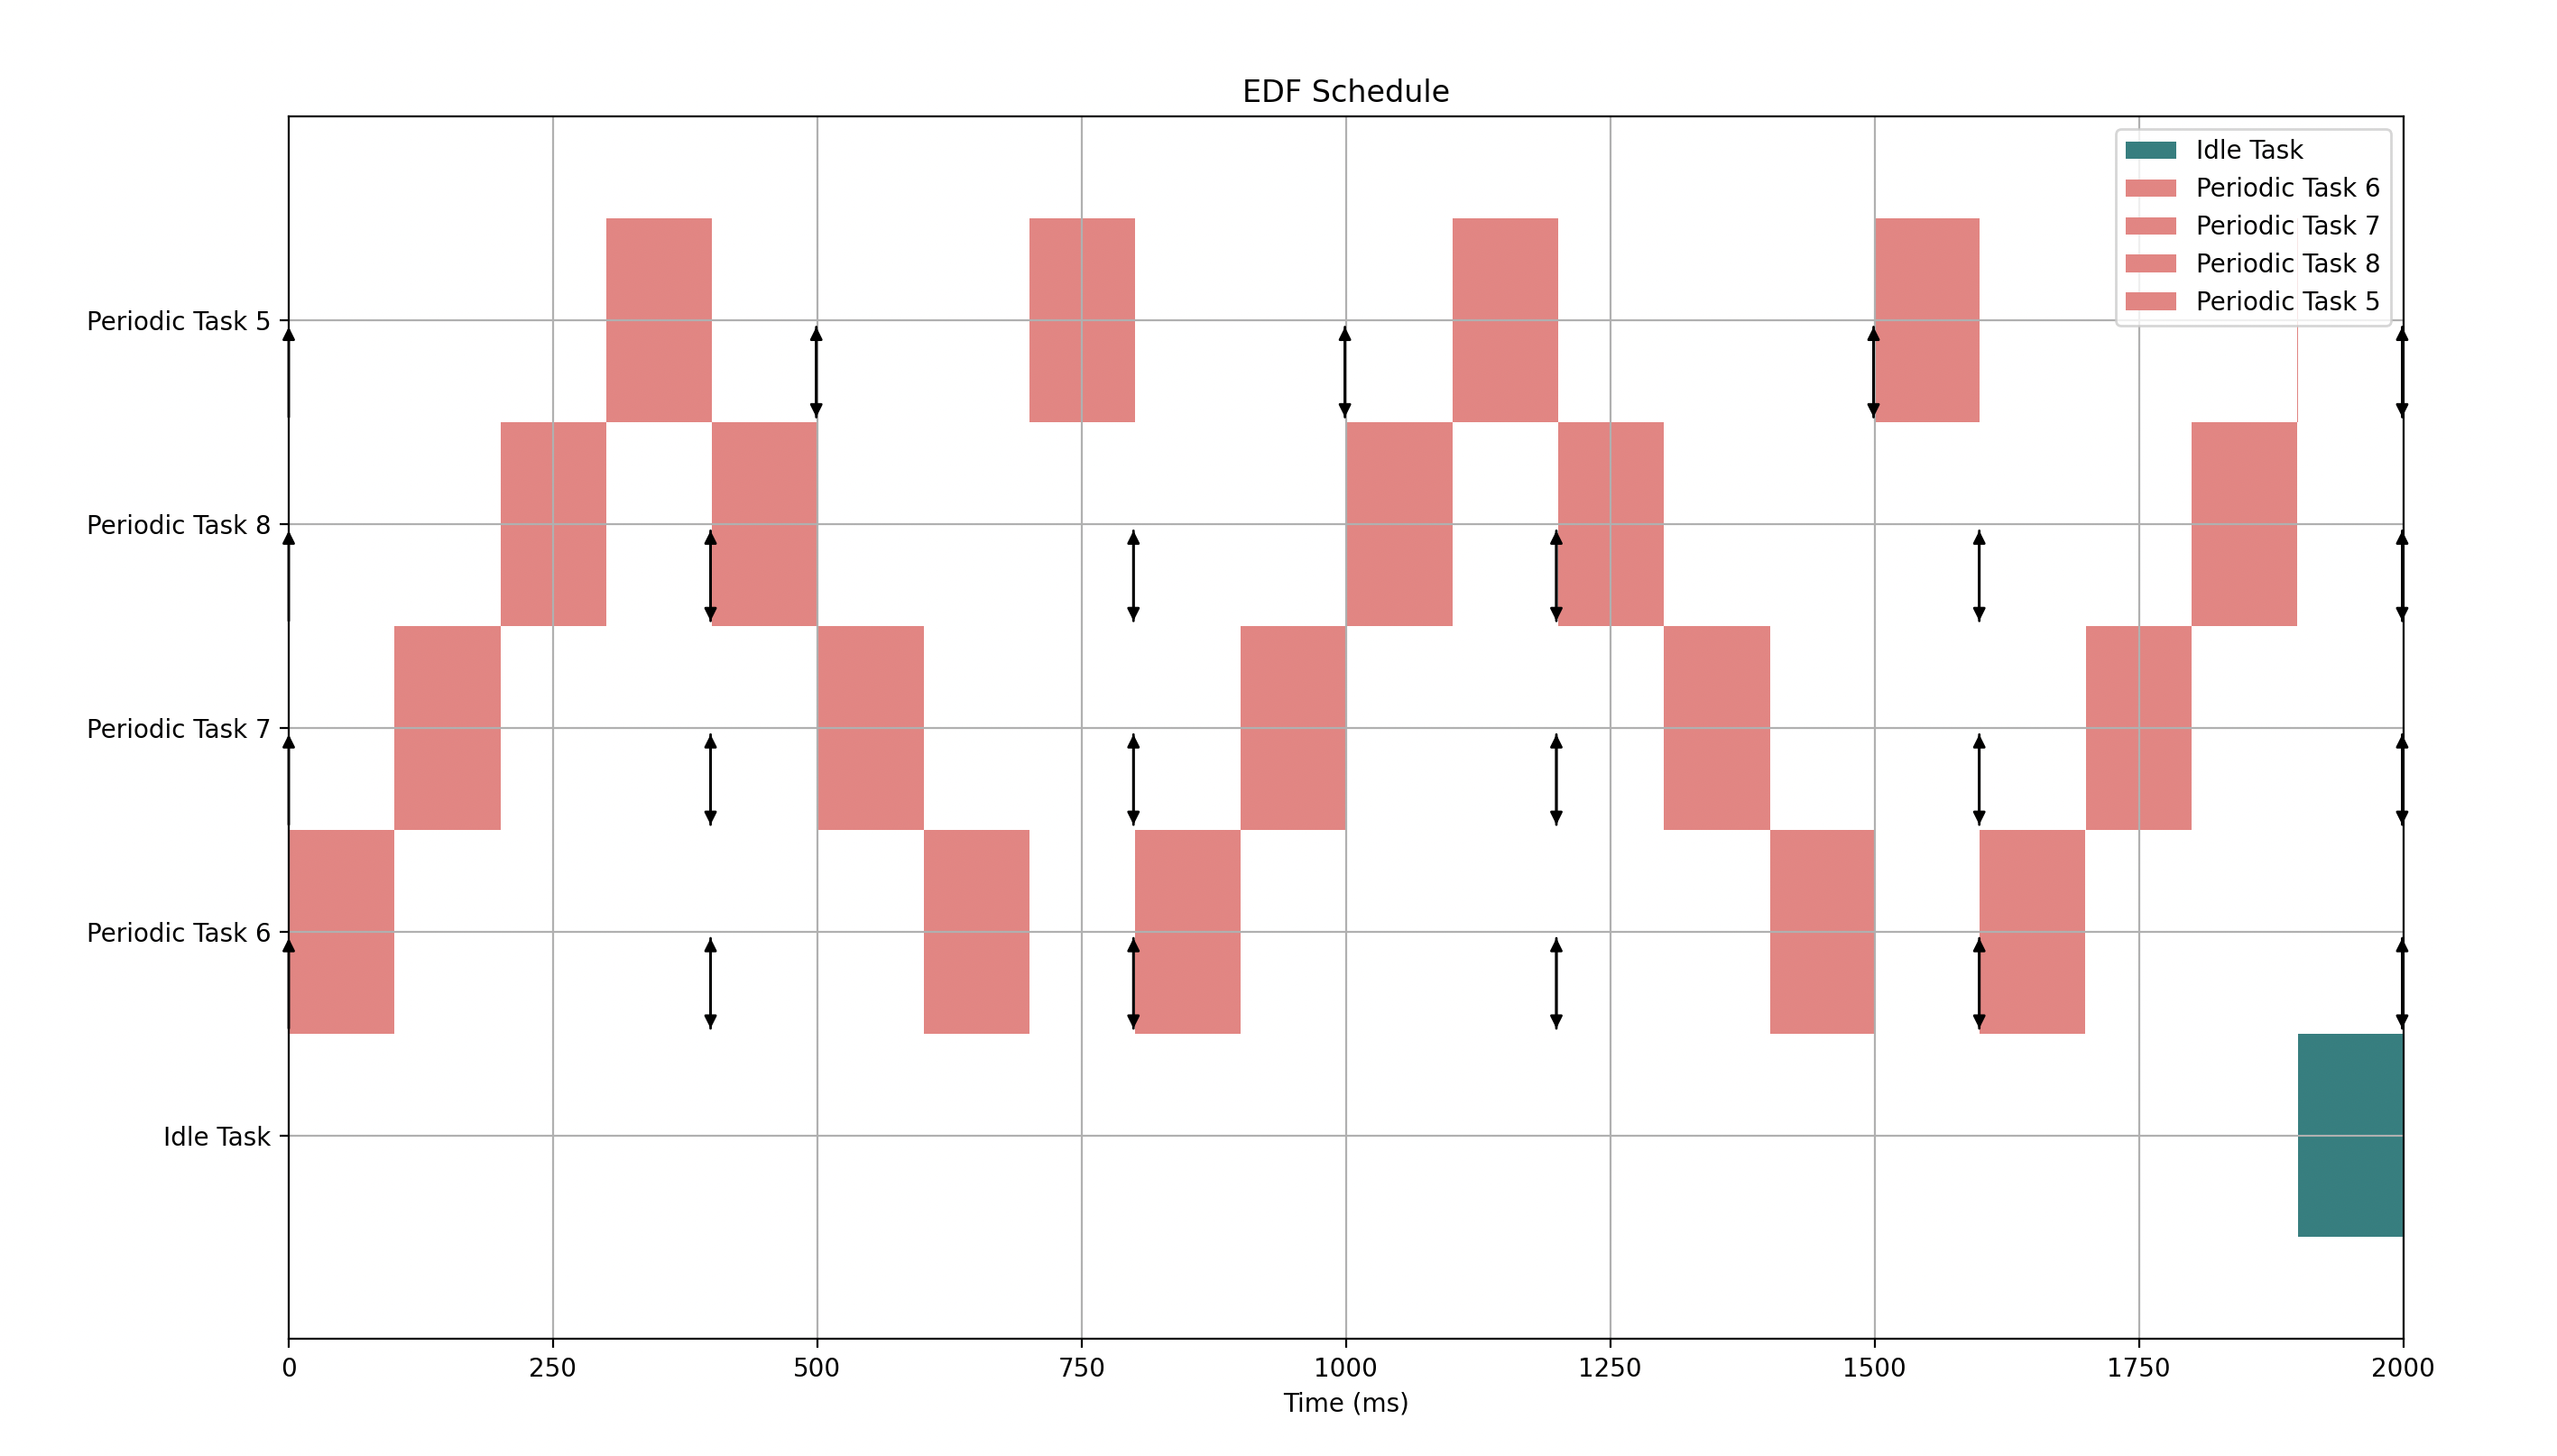
\includegraphics[scale = 0.25]{figures/Ex5_mod_4P.png}}
		\label{Fig5}
	\end{figure*}
	}%end footnote size	
\end{frame}

% \InsertTitle{}
% Example 6: 3 periodic, phase shifted
\begin{frame}{\small{EDF results: 3 periodic tasks with phase shifts}}
	\footnotesize{
	\begin{table}[ht]\label{table7}
		\hskip-7.0cm\begin{tabular}{lcccccl}\toprule
		\hline
		 & ${\tau_{5}}$ & ${\tau_{6}}$ & ${\tau_{7}}$\\\midrule
		\hline
		${\phi_{i}}$ & 100 & 0 & 200\\
		$a_{i}$ & 0 & 0 & 0\\
		$c_{i}$ & 100 & 200 & 100\\
		$P_{i}$ & 400 & 800 & 400\\
		$D_{i}$ & 400 & 800 & 400\\\bottomrule
		\hline
	\end{tabular}
\end{table}

Utilization factor \\
\hfill\break
$U_{p} = \sum \dfrac{C_{i}}{P_{i}}\\
\hspace{0.2in} = \dfrac{100}{400} + \dfrac{200}{800} + \dfrac{100}{400} = 0.75}$
\end{frame}

\begin{frame}
\begin{figure*}
	\centerline{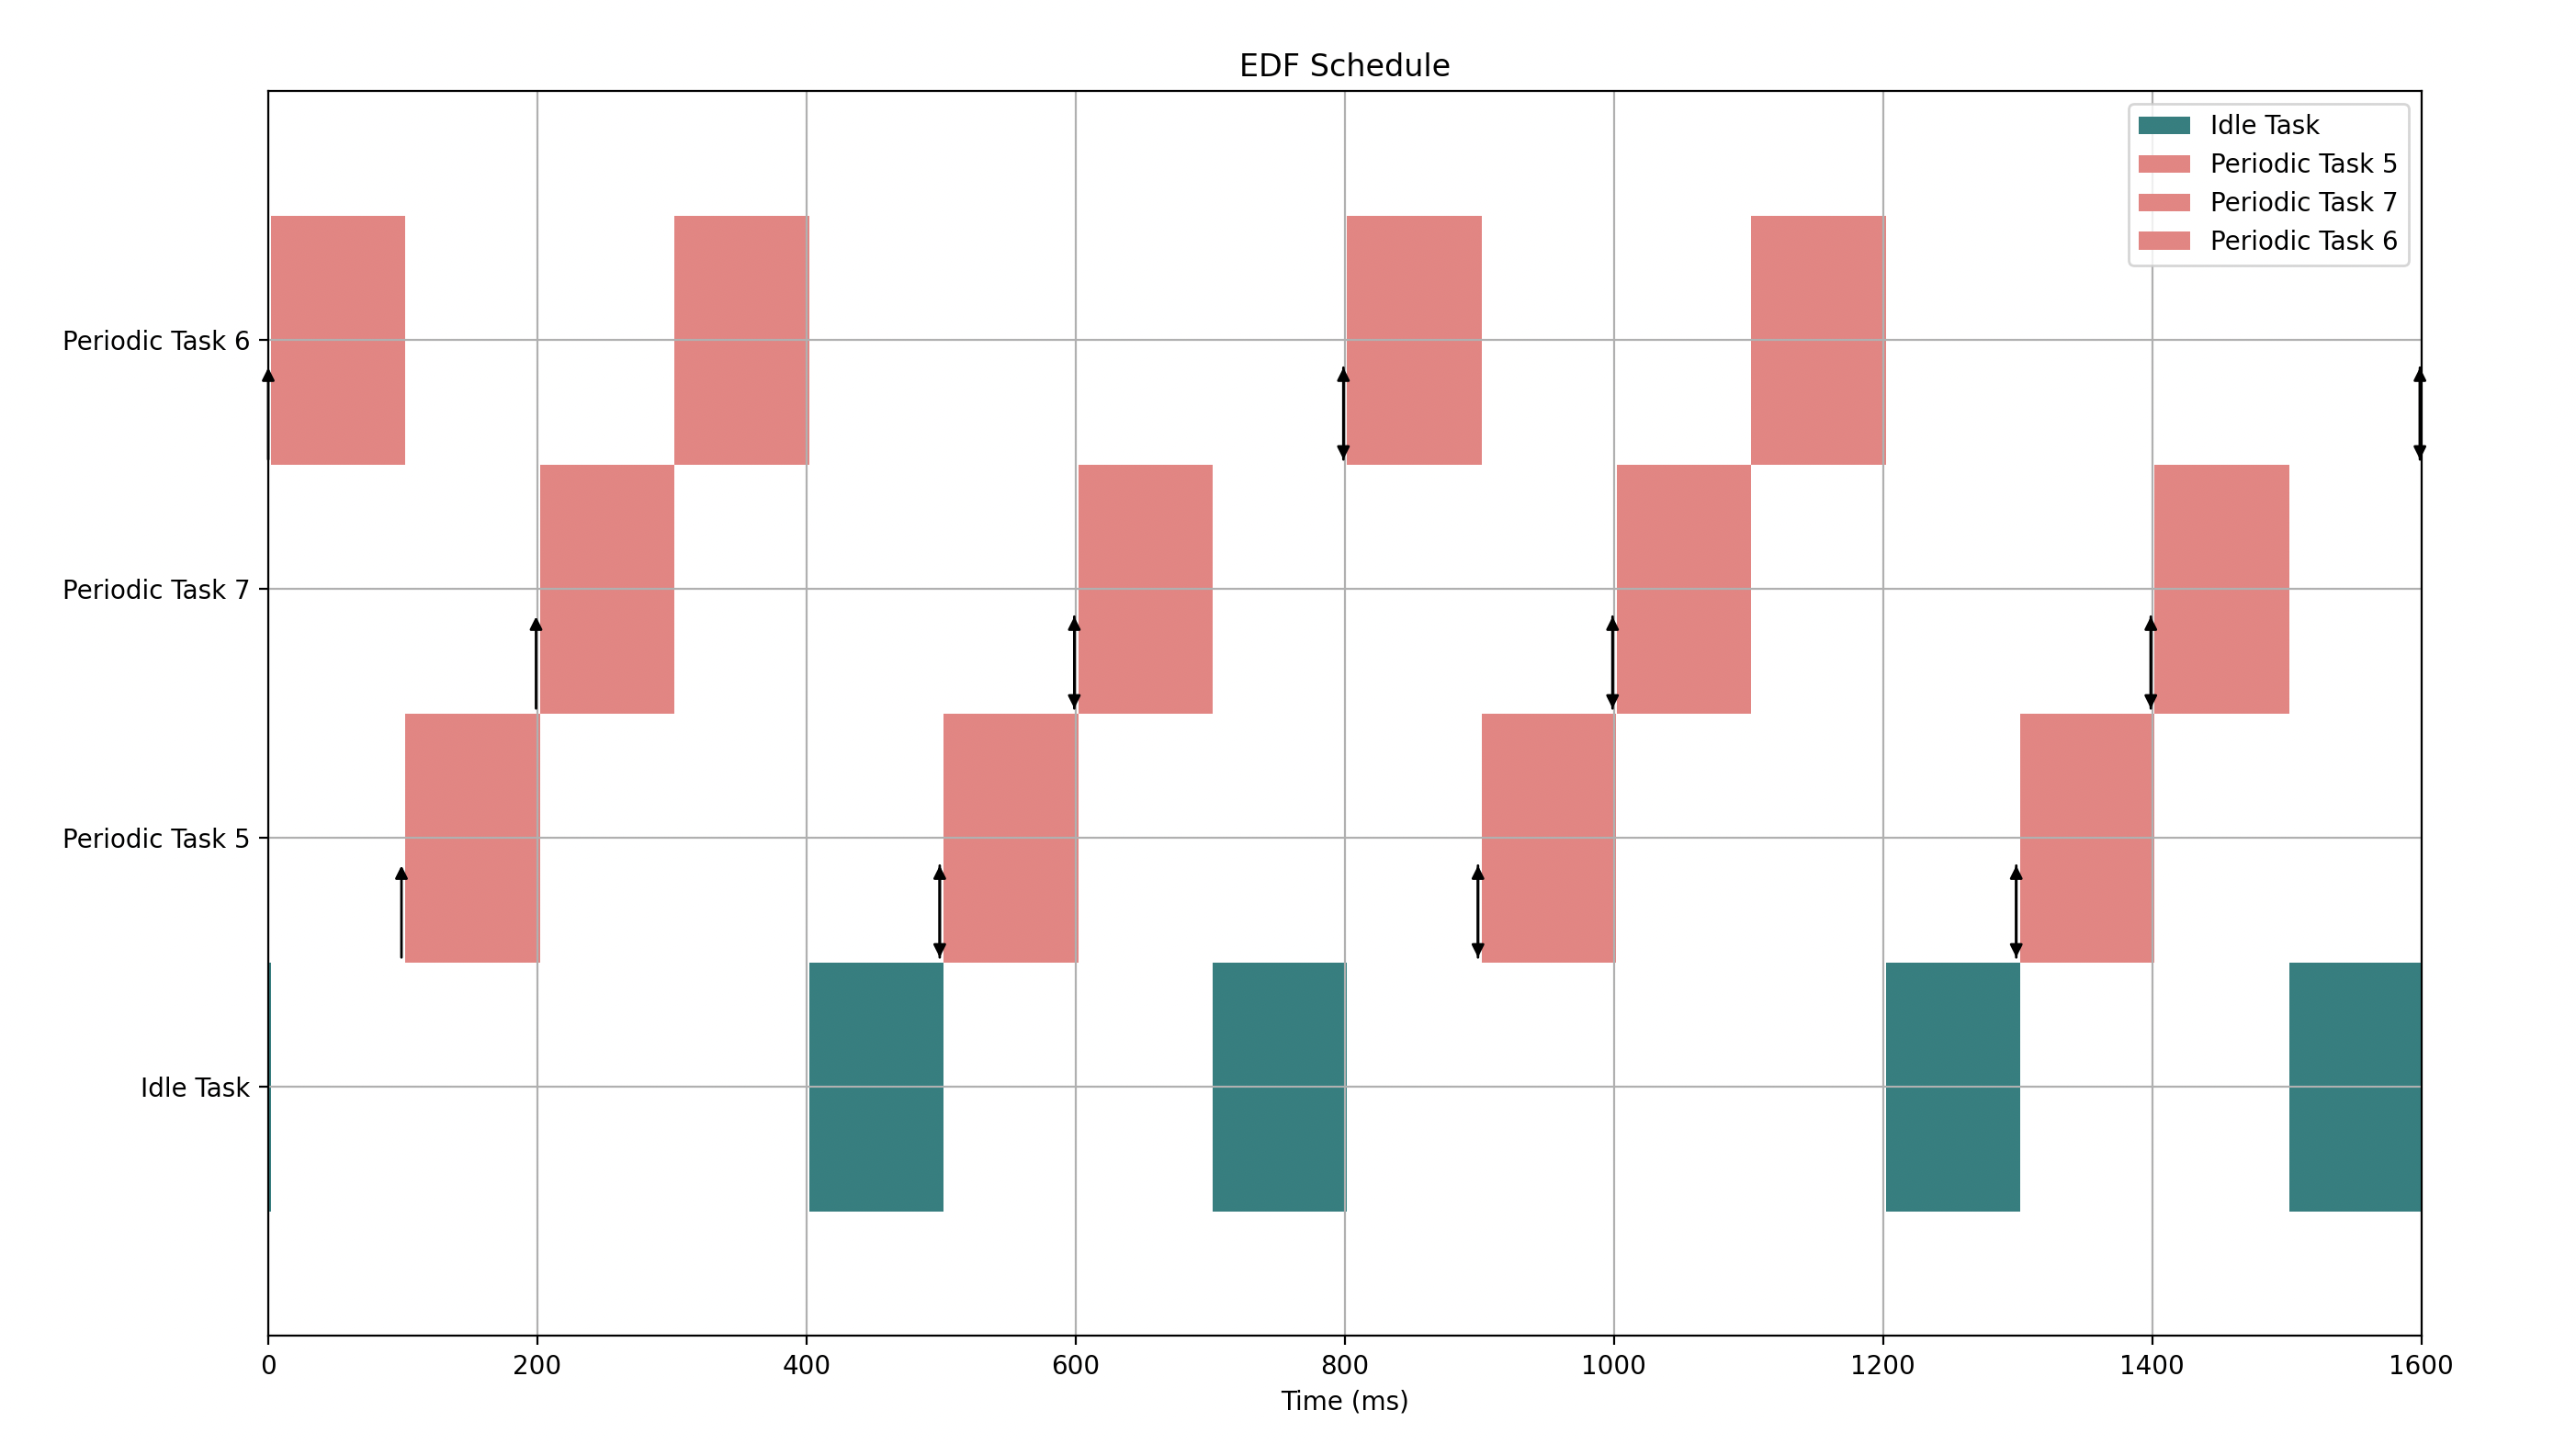
\includegraphics[scale = 0.25]{figures/Ex6_3P.png}}
	\label{Fig6}
\end{figure*}
\end{frame}

% Example 8: 3 periodic, 2 aperiodic
\begin{frame}{\small{EDF results: 3 periodic, 2 aperiodic tasks}}
		\footnotesize{
		\begin{table}[ht]\label{table8}
			\hskip-5.0cm\begin{tabular}{lcccccl}\toprule
			\hline
			 & ${\tau_{5}}$ & ${\tau_{6}}$ & ${\tau_{7}}$ & ${J_{14}}$ & ${J_{15}}$\\\midrule
			\hline
			${\phi_{i}}$ & 0 & 0 & 0 &  &  \\
			$a_{i}$ & 0 & 0 & 0 & 200 & 800 \\
			$c_{i}$ & 100 & 200 & 100 & 100 & 100 \\
			$P_{i}$ & 400 & 800 & 400 &  &  \\
			$D_{i}$ & 400 & 800 & 400 &  &  \\\bottomrule
			\hline
		\end{tabular}
	\end{table}

	Utilization factor and aperiodic deadlines for TBS\\
	\hfill\break
	$U_{p} = \dfrac{100}{400} + \dfrac{200}{800} + \dfrac{100}{400} = 0.75$
	
	$U_{s} = 0.25$
	
	$D_{i} = max(a_{i} + d_{i-1}) + \dfrac{C_{i}}{U_{s}}$\\
	$D_{14} = 200 + \dfrac{100}{0.25}\\
	\hspace{0.2in} = 600$

	$D_{15} = 800 + \dfrac{100}{0.25}\\
	\hspace{0.2in} = 1200}$
\end{frame}

\begin{frame}
	\begin{figure*}
		\centerline{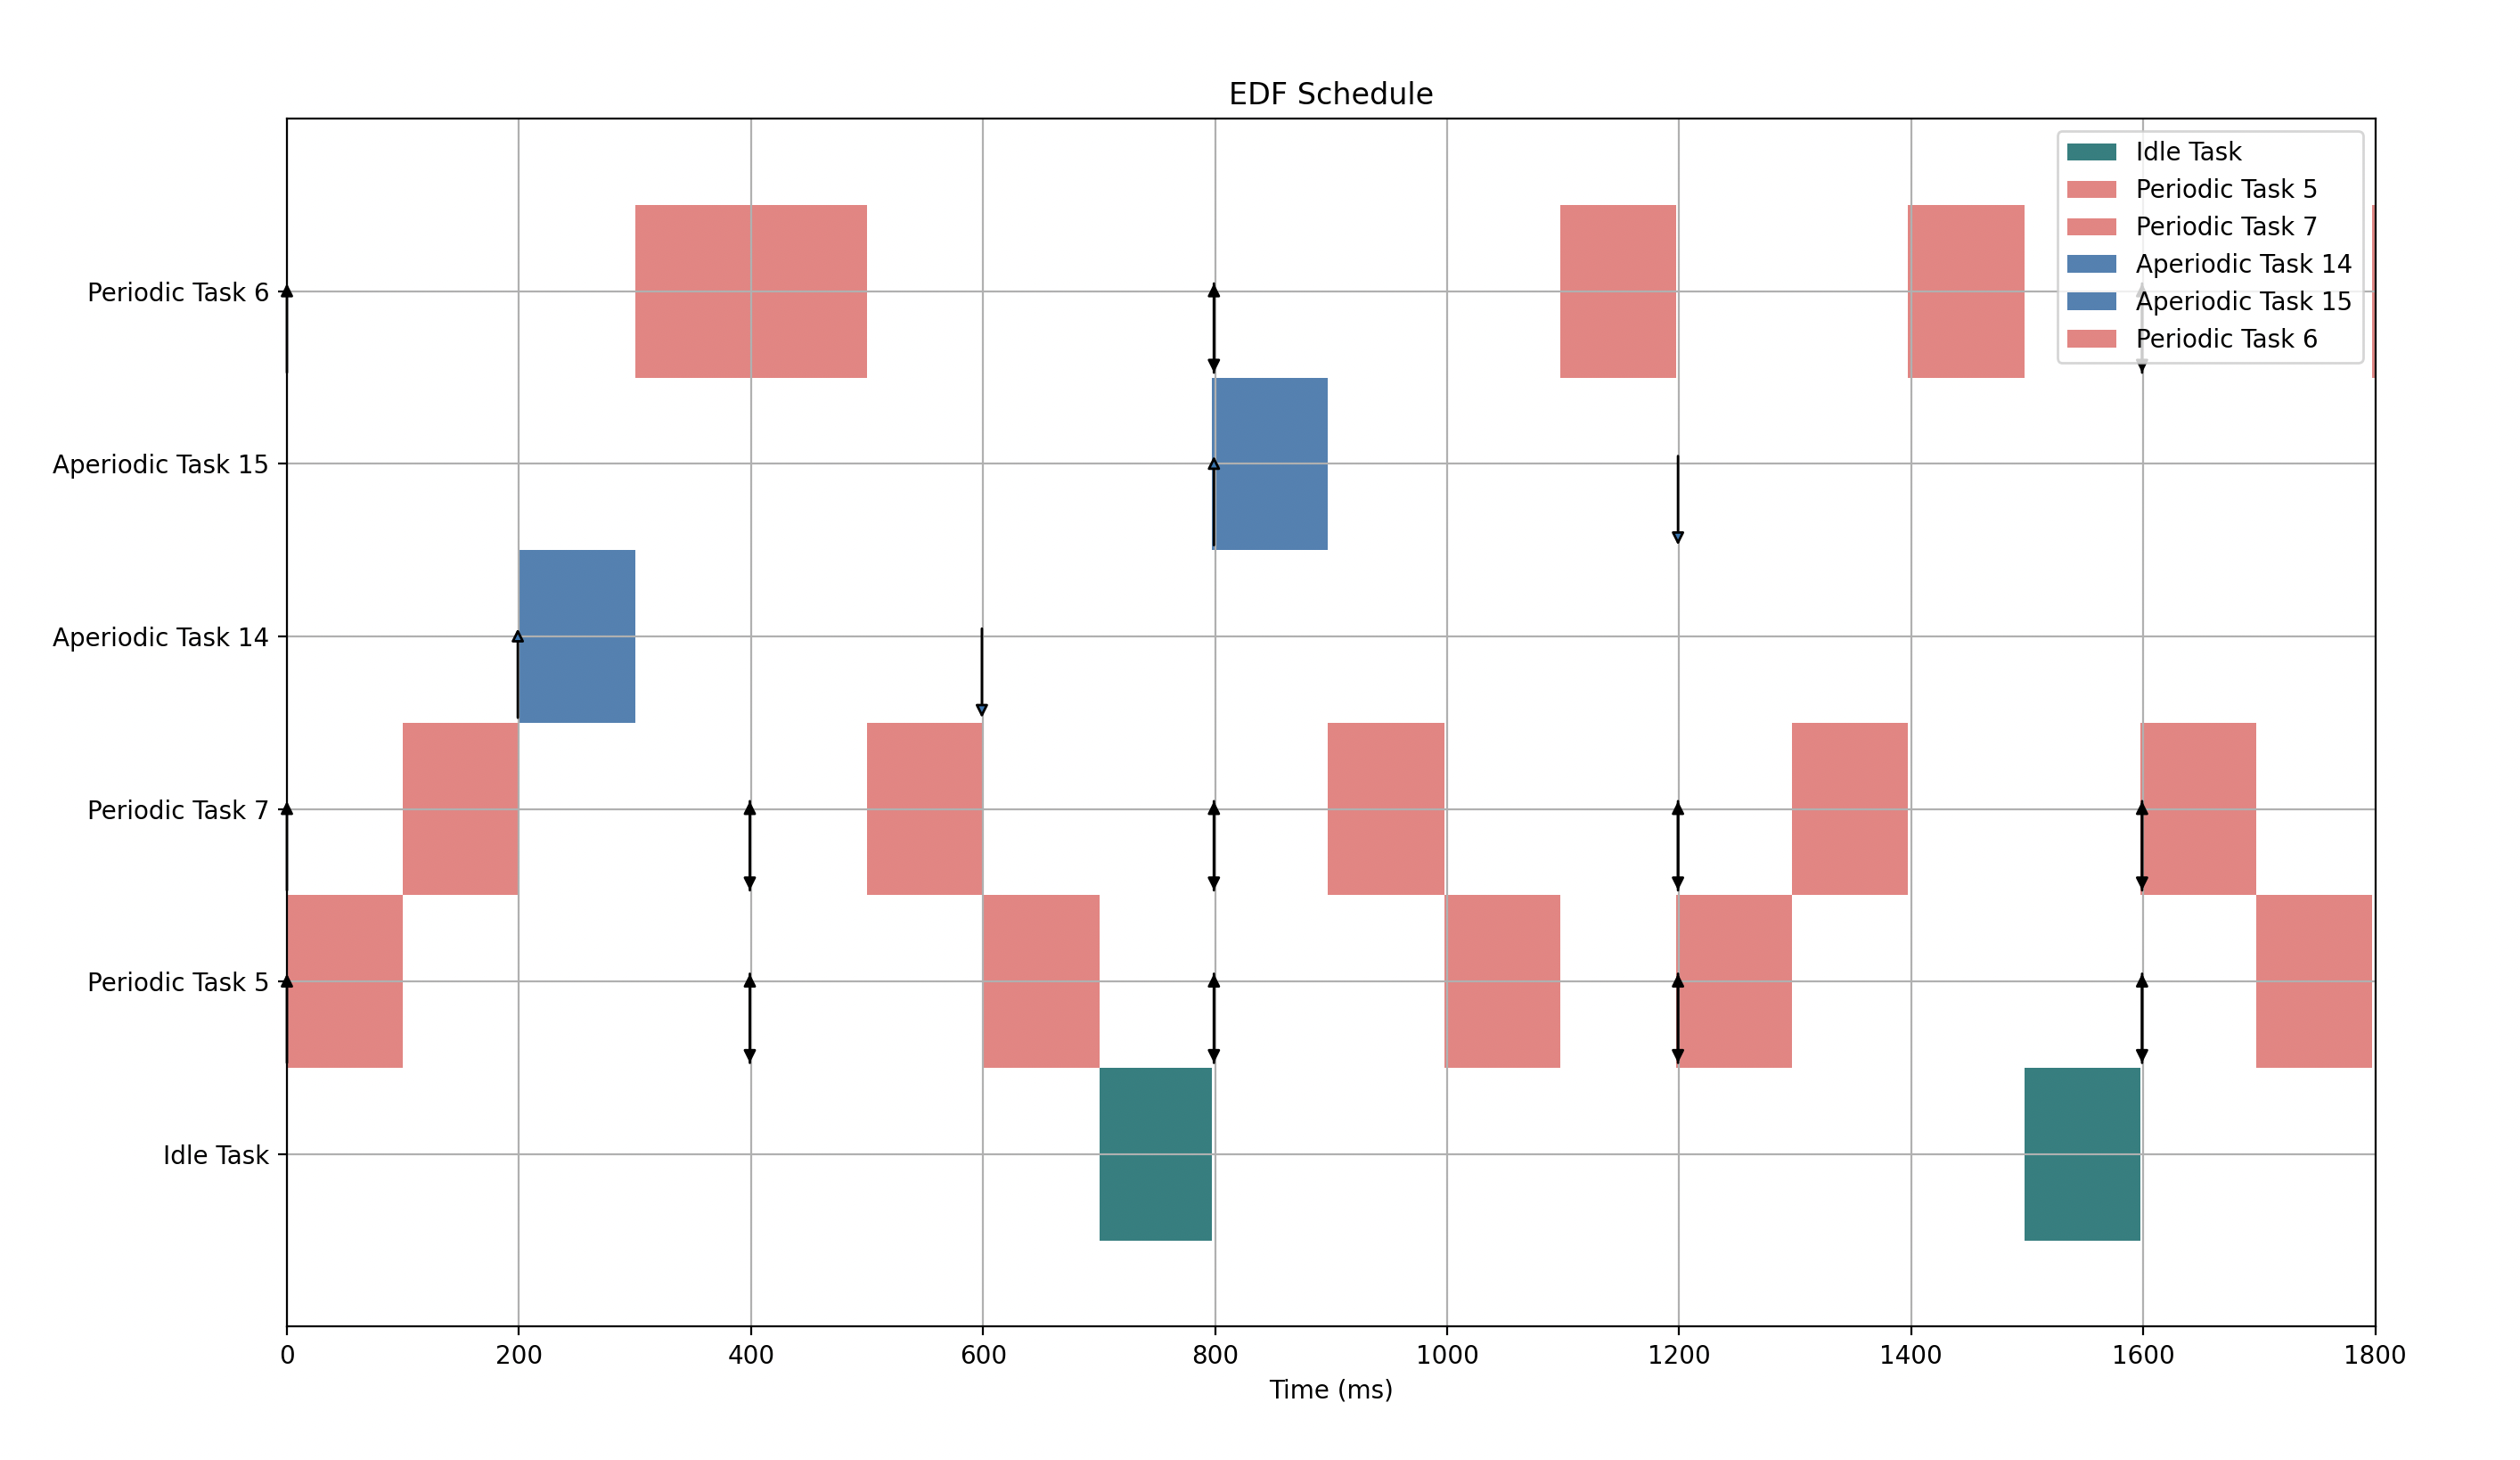
\includegraphics[scale = 0.25]{figures/Ex8_3P_2AP.png}}
		\label{Fig8}
	\end{figure*}
\end{frame}

% Example 10: 3 periodic
\begin{frame}{\small{EDF results: 3 periodic, 2 aperiodic tasks, with deadline overflows}}
	\footnotesize{
	\begin{table}[ht]\label{table10}
		\hskip-5.0cm\begin{tabular}{lcccccl}\toprule
		\hline
		 & ${\tau_{5}}$ & ${\tau_{6}}$ & ${\tau_{7}}$& ${J_{14}}$ & ${J_{15}}$\\\midrule
		\hline
		${\phi_{i}}$ & 0 & 0 & 0 &  & \\
		$a_{i}$ & 0 & 0 & 0 & 200 & 800\\
		$c_{i}$ & 100 & 100 & 200 & 100 & 100\\
		$P_{i}$ & 300 & 300 & 400 \\
		$D_{i}$ & 300 & 300 & 400 \\\bottomrule
		\hline
	\end{tabular}
\end{table}

Utilization factor and aperiodic deadlines for TBS\\
\hfill\break
$U_{p} = \dfrac{100}{300} + \dfrac{100}{300} + \dfrac{200}{400} = 1.167$

\hfill\break
$U_{s} = 0$ (Aperiodic tasks not scheduled)\\
\hfill\break

Expected overflow at 900ms.\\
Additionally detected at 1200ms, due to overhead in deleting ${\tau_{5}}$.

}
\end{frame}

\begin{frame}
\begin{figure*}
	\centerline{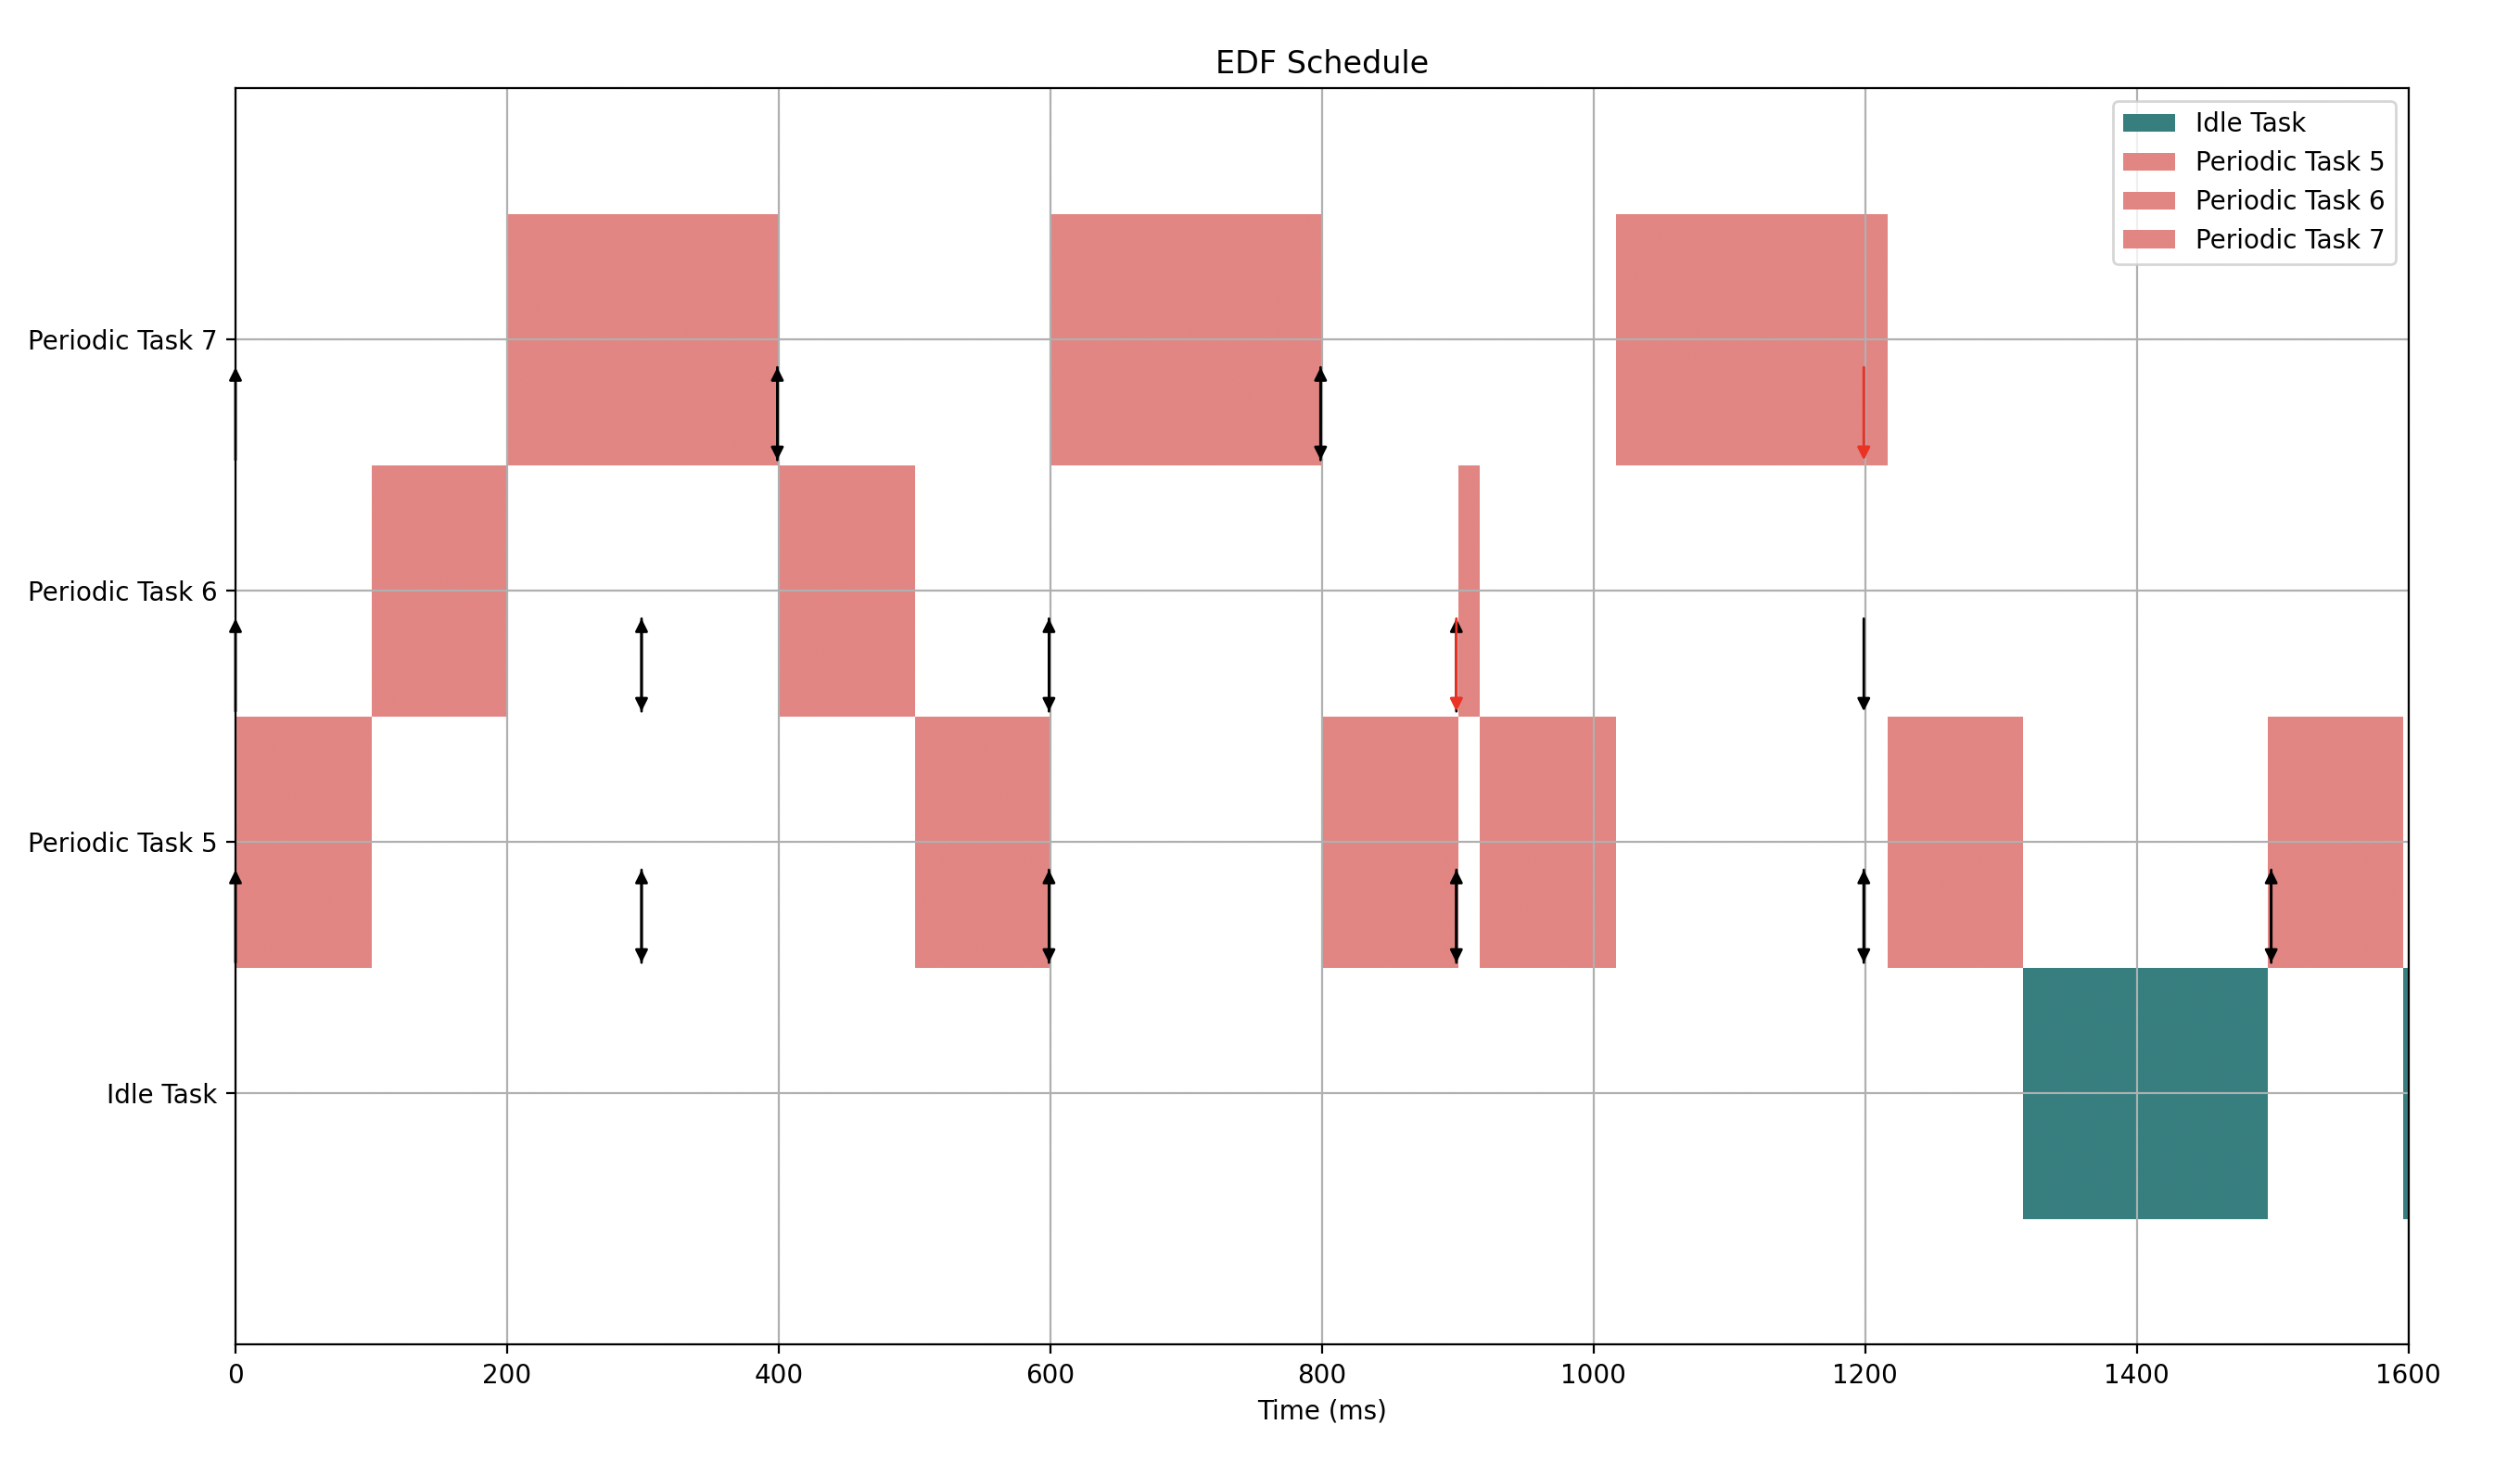
\includegraphics[scale = 0.25]{figures/Ex10_3P_DL.png}}
	\label{Fig10}
\end{figure*}
\end{frame}


\begin{frame}{\small{References}}
	\footnotesize{
		\begin{itemize}
			\item[$\bullet$] [1] R. Kase, Efficient Scheduling library for FreeRTOS (Master Thesis), KTH Stockholm, 2016.\\
			\item[$\bullet$] [2] ESP-FreeRTOS APIs, https://docs.espressif.com/projects/esp-idf/en/latest/esp32/api-reference/system/freertos.html\\
			\item[$\bullet$] [3] C. Scholl, Real Time Operating Systems and Worst Case Execution Times (Lecture Notes), University of Freiburg, 2022.\\
			
		\end{itemize}
	}
\end{frame}


\bibliographystyle{plain}

\end{document}
